\chapter{Конструкторский раздел}

В данном разделе приведены ключевые алгоритмы использованные при написании драйвера сканера отпечатка пальца.

\section{Структура ПО}

Разрабатываемое ПО состоит из драйвера сканера отпечатка пальца и пользовательского приложения для тестирования работы драйвера.

\begin{figure}[h!]
    \centering
    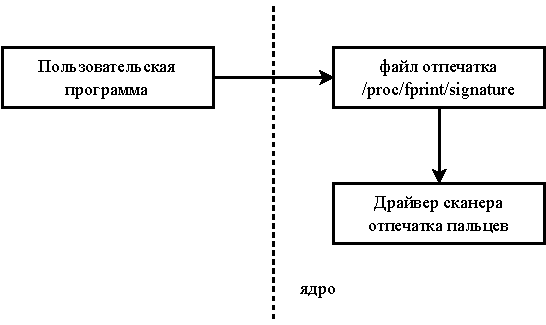
\includegraphics[width=0.9\textwidth]{img/structure-po}
    \caption{Структура ПО}
\end{figure}

\section{Алгоритм обработки URB}

На рисунке \ref{fig:init} представлен алгоритм инициализации TLS соединения с устройством. PKS -- pre-shared key cichersuites -- предварительный общий ключ безопасности используемый в качестве сертификата.

\begin{figure}[h!]
    \centering
    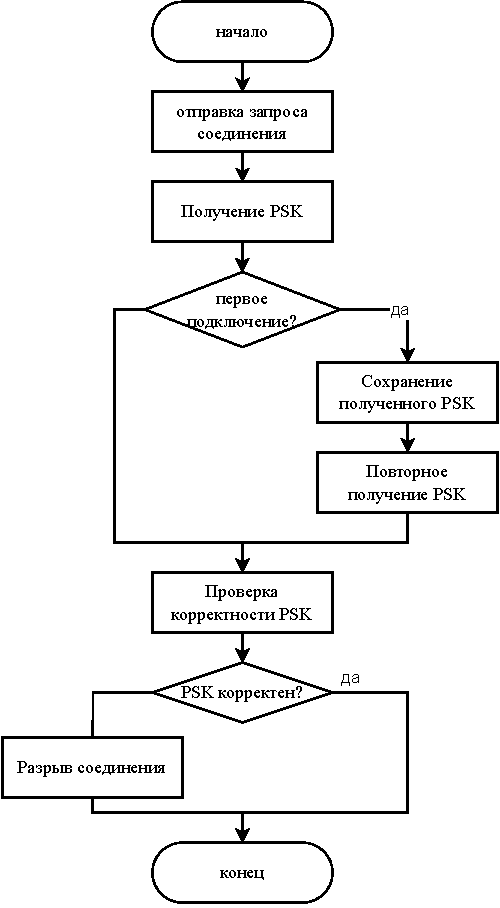
\includegraphics[width=0.7\textwidth]{img/init}
    \caption{Алгоритм инициализации соединения}
    \label{fig:init}
\end{figure}
